\chapter{Mecánica}

\section{Objetivo y Necesidad}

En el departamento de Ingeniería de la Universidad de Monterrey, existe una línea de tradición en el diseño automotríz, ésta cuenta ya con un auto de hidrógeno, y su siguiente paso es el Vehículo Autónomo Supermilla. El VAS es un proyecto que consiste en modificar el vehículo supermilla (Figura 1) y convertirlo en un auto con dirección autónoma, esto es, se controlará por una computadora que tomará las decisiones para el posicionamiento angular de las llantas. Una de las etapas de este nuevo proyecto es la generación de una dirección controlada eléctricamente (drive by wire), para lo cual se requiere de la implementación de un mecanismo que soporte el control de la dirección con un motor a máximo 24VDC.

\begin{figure}
\centering
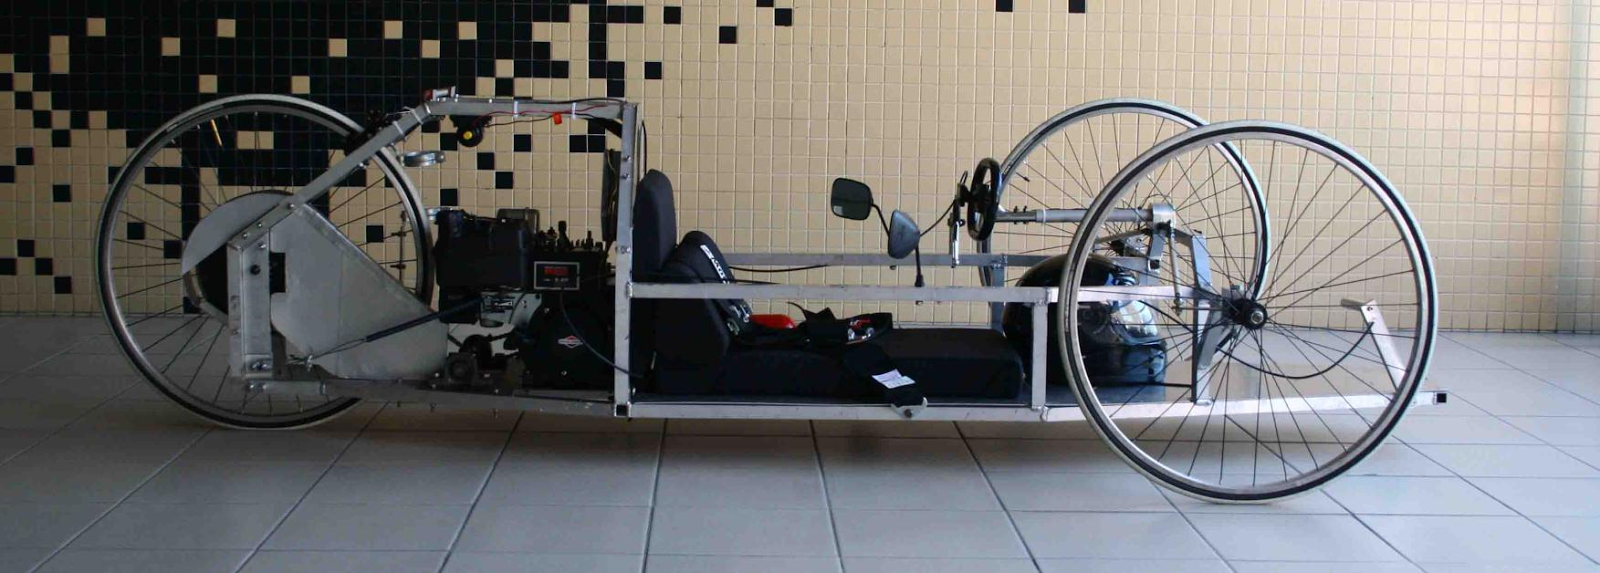
\includegraphics[width=4.5in]{fotos/inicial}
\caption{Vehículo supermilla en su estado inicial}
\label{fig:fotos:inicial}
\end{figure}

\begin{table}[h]
\centering
\begin{tabular}{@{}lcc@{}}
\toprule
\multicolumn{1}{c}{\textbf{Parámetro}} & \textbf{Magnitud} & \textbf{Unidad} \\ \midrule
Potencia                               & 0.17              & HP              \\
Velocidad angular                      & 1800              & RPM             \\
Torque                                 & 0.49              & lb.ft           \\
Torque                                 & 5.84              & lb.in           \\
FS                                     & 2.00              & N/A             \\
Longitud del lado de la base           & 2 5/8             & pulgada         \\
Diámetro de la flecha                  & 1/2               & pulgada         \\
Longitud motor sin flecha              & 7 7/8             & pulgada         \\
Longitud flecha                        & 1 1/2             & pulgada         \\ \bottomrule
\end{tabular}
\caption{Parámetros de interés del motor DAYTON 900-3140-050.}
\label{tab:parametros_motor}
\end{table}

\begin{table}[h]
\centering
\begin{tabular}{@{}lcc@{}}
\toprule
\multicolumn{1}{c}{\textbf{Parámetro}} & \textbf{Magnitud} & \textbf{Unidad} \\ \midrule
Altura al centro de la flecha          & 13.80             & pulgadas        \\
Revoluciones deseadas                  & 1.5               & rev/s           \\
Revoluciones deseadas                  & 90                & RPM             \\
Fuerza necesaria para girar dirección  & 55                & N               \\
Torque necesario para girar dirección  & 38.94             & lb.in           \\ \bottomrule
\end{tabular}
\caption{Algunos parámetros de interés del mecanismo de dirección.}
\label{tab:parametros_direccion}
\end{table}

\begin{table}[h]
\centering
\begin{tabular}{@{}lccc@{}}
\toprule
\textbf{Componente} & \multicolumn{1}{l}{\textbf{RPM}} & \multicolumn{1}{l}{\textbf{Torque (lb.in)}} & \multicolumn{1}{l}{\textbf{Relación}} \\ \midrule
Piñón motor         & 1800                             & 5.84                                        & 4                                     \\
Engrane             & 450                              & 23.34                                       & 1                                     \\
Piñón               & 450                              & 23.34                                       & 4                                     \\
Engrane             & 112.5                            & 93.37                                       & 1                                     \\
Sprocket            & 112.5                            & 93.37                                       & 1.25                                  \\
Sprocket            & 90                               & 116.71                                      & \textbf{20}                           \\ \bottomrule
\end{tabular}
\caption{Reducción a través de los componentes de la transmisión.}
\label{tab:reduccion}
\end{table}

\begin{table}[h]
\centering
\begin{tabular}{@{}ll@{}}
\toprule
Parámetro       & Magnitud \\ \midrule
Dientes driver  & 12       \\
Dientes driven  & 15       \\
Pitch cadena    & 0.50"    \\
Center distance &          \\ \bottomrule
\end{tabular}
\caption{Datos de la transmisión por sprockets}
\label{tab:parametros_sprockets}
\end{table}

\begin{table}[h]
\centering
\begin{tabular}{@{}ll@{}}
\toprule
Parámetro           & Magnitud \\ \midrule
C                   & 20.7042  \\
S                   & 27       \\
D                   & 3        \\
K                   & 0.23     \\
Length  (pitches)   & 54.92    \\
Length (55 pitches) &          \\ \bottomrule
\end{tabular}
\caption{Resultados para la transmisión por sprockets}
\label{tab:resultados_sprockets}
\end{table}

% Please add the following required packages to your document preamble:
% \usepackage{booktabs}
\begin{table}[h]
\centering
\begin{tabular}{@{}lccc@{}}
\toprule
\multicolumn{1}{c}{\textbf{Componente}} & \textbf{No. de parte}    & \textbf{Cantidad} & \textbf{Precio unitario} \\ \midrule
Engrane 18 dientes                      & S2418 (Martin)           & 2                 & 300.00                   \\
Engrane 72 dientes                      & S2472 (Martin)           & 2                 & 980.00                   \\
Sprocket 12 dientes                     & 41B12 (Martin)           & 1                 & 174.00                   \\
Sprocket 15 dientes                     & 41B15 (Martin)           & 1                 & 194.88                   \\
Cadena                                  & Roller chain ANSI no. 40 & 1                 & 290.00                   \\
Balero                                  & 6203-1/2 2RS             & 3                 & 50.00                    \\
Balero                                  & 608-2RS 8-22-7           & 1                 & 25.00                    \\
Flecha                                  & Acero 1018 1/2"          & 1                 & 8.00                     \\
Flecha                                  & Acero 1018 3/8"          & 1                 & 5.00                     \\
Flecha                                  & Acero 1018 1/2"          & 1                 & 12.25                    \\
Flecha                                  & Acero 1045 1"            & 1                 & 117.60                   \\
Solera                                  & Acero 1018               & 1                 & 232.00                   \\ \bottomrule
\end{tabular}
\caption{Componentes utilizados en el mecanismo de dirección y sus precios.}
\label{tab:componentes_mecanicos}
\end{table}

\begin{table}[h]
\centering
\scriptsize
\begin{tabular}{@{}lcccccccc@{}}
\toprule
\multicolumn{1}{c}{\textbf{Criterios}} & \textbf{Parámetro} & \textbf{Meta}   & \textbf{Importancia}               & \textbf{C1} & \textbf{C2} & \textbf{C3} & \textbf{C4} & \textbf{C5} \\ \midrule
Ergonomía                              & Comodidad          & Aceptable       & 2                                  & 3           & 3           & 9           & 9           & 1           \\
Espacio ocupado                        & CC                 & \textless 64000 & 8                                  & 3           & 3           & 9           & 9           & 3           \\
Estabilidad                            & altura (cm)        & 0               & 9                                  & 9           & 9           & 1           & 1           & 9           \\
Manufacturabilidad                     & Complejidad        & Baja            & 5                                  & 9           & 3           & 3           & 9           & 1           \\
Conveniencia montaje                   & Complejidad        & Baja            & 4                                  & 3           & 1           & 3           & 3           & 9           \\
Eficiencia de transmisión              & \% out/in          & Alta            & 10                                 & 3           & 3           & 9           & 3           & 9           \\
\multicolumn{3}{l}{\multirow{2}{*}{}}                                         & \multicolumn{1}{r}{\textbf{Ponderación}}    & 198         & 160         & 216         & 186         & 238         \\
\multicolumn{3}{l}{}                                                          & \multicolumn{1}{r}{\textbf{Lugar relativo}} & 3           & 5           & 2           & 4           & 1           \\ \cmidrule(l){4-9} 
\end{tabular}
\caption{Resultados de la evaluación.}
\label{tab:evaluacion_conceptos}
\end{table}

El mecanismo debe cumplir la función de transmitir la energía de rotación del motor (controlada) para efectuar el movimiento de las llantas exigiendo la menor cantidad de torque del motor, además debe ser lo suficientemente compacto para no afectar de manera considerable el espacio disponible para el conductor. El diseño del mecanismo debe hacerse considerando que el mecanismo es un subsistema de una máquina que responderá de manera autónoma al entorno, por lo que se debe considerar:

\begin{itemize}
\item Minimizar el torque necesario para moverlo (bajar el precio del motor).
\item Minimizar el radio de giro del vehículo (permitirá mayor control del mismo).
\item Maximizar sensibilidad de giro (que se cambiar el ángulo de giro de la dirección rápidamente).
\end{itemize}

Creemos que este es problema que requiere de los conocimientos adquiridos en clase y una gran oportunidad para ponerlos en práctica. En la solución que se implementó se utilizan los siguientes componentes vistos en clase: engranes, sprockets, cadenas, flechas, bujes y baleros. A continuación se presenta el proceso de evaluación de conceptos, la selección de componentes y los resultados finales del trabajo realizado a lo largo del semestre.

\section{Problema y Propuestas}

\subsection{Delimitantes del problema}

Como el mecanismo se va a montar sobre un vehículo existente al cual se le busca hacer el menor número de modificaciones posibles es necesario tener en cuenta algunas dimensiones actuales del vehículo, particularmente las que están cerca del mecanismo de la dirección. Además ya se seleccionó un motor de corriente directa para la aplicación y los datos necesarios del motor también se muestran en el documento presente.

El chasis del vehículo es una armadura de PTR de aluminio de 1”x1”x1/8” soldados para formar la estructura mostrada en la siguiente imagen, en donde también se muestran las dimensiones de mayor interés para nuestro proyecto.

\begin{figure}
\centering
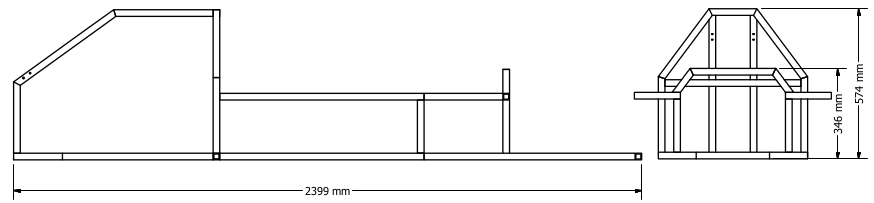
\includegraphics[width=4.5in]{dibujos/chasis}
\caption{Vistas lateral y frontal del vehículo}
\label{fig:fotos:chasis}
\end{figure}


A la altura de 346 mm mostrada en la imagen anterior se encuentra una chumacera de la que sale la flecha a la que está montado el volante con el que se conduce la dirección del vehículo. Las dimensiones de la chumacera se muestran a continuación.

\begin{figure}
\centering
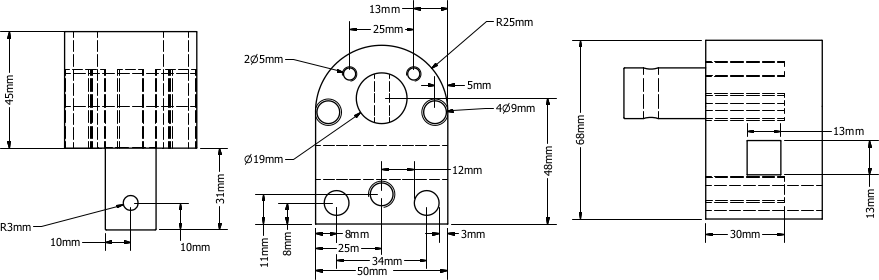
\includegraphics[width=4.5in]{dibujos/chumacera}
\caption{Vistas superior, lateral y frontal de la chumacera}
\label{fig:fotos:chumacera}
\end{figure}


La intención del proyecto actual es utilizar la misma chumacera y de ser posible la misma flecha, cortándola para ponerle un sprocket y así acoplarla a la transmisión de nuestro mecanismo para controlar la dirección eléctricamente. Después de una selección escogimos el motor DAYTON 900-3140-050. La apariencia y los parámetros del motor para nuestra aplicación se muestran a continuación:

\begin{figure}
\centering
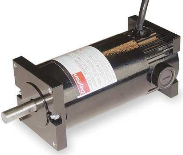
\includegraphics[width=4.5in]{fotos/motor}
\caption{Motor DAYTON 900-3140-050}
\label{fig:fotos:motor}
\end{figure}


*Tabla 1. Parámetros de interés del motor DAYTON 900-3140-050.

Siguiendo la decisión de mantener la flecha actual para no afectar el resto del mecanismo, remover el volante, cortarla y ponerle un sprocket para acoplarla a nuestra transmisión, los datos de interés del sistema dirección actual se muestran a continuación:

*Tabla 2. Algunos parámetros de interés del mecanismo de dirección.
*NOTAEstas mediciones se realizaron con el vehículo tripulado y en reposo, la fuerza necesaria disminuiría si el vehículo no estuviera tripulado y aumentaría al querer cerrar más una vuelta al estar en movimiento porque habría una fuerza centrífuga que empujaría las llantas hacia afuera.

\subsection{Propuestas evaluadas}
\subsubsection{Motor horizontalmente:}
El motor se encuentra horizontalmente sobre la superficie del VAS, requiere de dos sprockets para la transmisión de su potencia uno situado en su flecha y otro en la del mecanismo de dirección. 
\subsubsection{C1: Piñón y cremallera rectos}
La cremallera se pone con los dientes hacia abajo, permitiendo a la flecha del motor impulsarla desde abajo con un mecanismo de transmisión adecuado. El movimiento se transmite a las llantas por unas barras que estan unidas por medio de una articulación esferoidal a unos tornillos en los extremos de la cremallera. Es el más similar a la dirección actual (Figura 5).

*Figura 5. Dirección piñón-cremallera, dirección actual.

\subsubsection{C2: Articulado}

El movimiento se transmite a las llantas por unas barras unidas a un eslabón con articulaciones esferoidales que se hace girar impulsado por el motor y una transmisión intermedia (Figura 6).

*Figura 6. Dirección articulada.

\subsubsection{Motor Verticalmente:}
El motor se encuentra montado de tal manera que su flecha de encuentra de manera vertical
subsubsection{C3: Piñón y cremallera rectos}
La cremallera se pone con los dientes hacia el frente o la parte posterior del vehículo, permitiendo a la flecha del motor ser impulsada mediante un mecanismo de transmisión adecuado. El movimiento se transmite a las llantas por unas barras que estan unidas por medio de una articulación esferoidal a unos tornillos en los extremos de la cremallera.
\subsubsection{C4: Articulado}
El movimiento se transmite a las llantas por unas barras unidas a un eslabón con articulaciones esferoidales que se hace girar impulsado por el motor y una transmisión intermedia.
\subsubsection{Motor horizontalmente, cadena: C5: Motor horizontal, tren de engranajes y sprockets}
El movimiento se transmite a las llantas por unas barras unidas a un eslabón con articulaciones esferoidales que se hace girar impulsado por el motor y una transmisión intermedia.

\section{Evaluación de propuestas}
\subsection{Variables a Evaluar}
\begin{itemize}
\item Ergonomía: Posición en la que se encontrará el conductor.
\item Espacio ocupado.
\item Estabilidad: El motor se encuentra montado sobre soportes que resistan al peso del mismo y a las vibraciones del VAS.
\item Manufacturabilidad: Complejidad del diseño de las piezas involucradas.
\item Conveniencia de montaje: estará medidas en la cantidad de modificaciones mecánicas que habrán que hacerse al VAS.
\item Eficiencia de transmisión.
\end{itemize}
\subsection{Listado de Conceptos}
\begin{itemize}
\item C1: Horizontal- Piñón y cremallera rectos
\item C2: Horizontal- Articulado
\item C3: Vertical- Piñón y cremallera rectos
\item C4: Vertical- Articulado
\item C5: Horizontal - Tren engranajes y sprocket
\end{itemize}

*Tabla 3. Simbología de ponderación para la evaluación.
*Tabla 4. Resultados de la evaluación.

\section{Concepto Ganador}
La evaluación de conceptos arrojó como mejor opción al concepto número cinco (Tabla 4). Simplificadamente se podría decir que se estará cambiando el volante por el sprocket del nuevo mecanismo.

\subsection{Diseño conceptual}

Tomando en cuenta las restricciones espaciales se llegó a una propuesta como la que se mostró en la Figura 7. El cuadro representa al motor, en cuya flecha va el primero de los dos pares iguales de engranajes del pequeño tren de engranajes de la solución. En la salida de dicho tren de engranajes se coloca un sprocket que transporta la potencia hasta la altura deseada. Los detalles de los componentes seleccionados se pueden encontrar en la siguiente sección de este documento. El uso de sprockets se hizo pensando en que la cadena haría sencillo subir la potencia hasta la dirección del vehículo, en contraste con el uso de engranes, para los que seguramente hubiéramos tenido que proponer muchos más componentes o acercar el motor a la flecha de la dirección. Esto tiene, además de la ventaja de aprovechar el mecanismo existente, la ventaja de que el motor y los componentes de reducción quedan a la altura de la base del vehículo, que es la ubicación más firme que podrían tener. 

Figura 7. Diagrama conceptual de la solución ganadora.
Esta es una solución que cumple satisfactoriamente con las limitantes del problema y decidimos implementarla siguiendo los resultados que obtuvimos de nuestro proceso de selección de conceptos.
\section{Selección de Componentes Mecánicos}
\subsection{Diseño de reducción}
De la definición del problema se obtiene que la relación de reducción de velocidad del sistema es de 20:1.

*RPMINRPMOUT=180090=20

La reducción seleccionada entre los componentes de la transmisión de la Figura 7 se muestra en la siguiente tabla:

*Tabla 5. Reducción a través de los componentes de la transmisión

En la tabla anterior se demuestra que se cumple con la relación de reducción que se quiere tener en el problema y se observa que el torque de salida es tres veces el torque necesario para hacer girar el vehículo cuando hay una persona en él y éste no está en movimiento. Además, en la Figura 7 de la transmisión propuesta se observa que la solución cumple con las restricciones espaciales del problema.

\subsection{Proceso de selección de engranes}
La primera recomendación en el catálogo de Browning es para el número mínimo e ideal de dientes. El mínimo, para el ángulo de presión de 14.5° es de 16 y el ideal es de 20. Nuestra selección fue de 18.

*Tabla 6. Recomendaciones para el número de dientes.

Nosotros buscamos una razón de reducción de velocidad de 4:1 y no tenemos restricción de distancia entre centros porque nosotros vamos a hacer el mecanismo final. Por lo tanto solamente tenemos que buscar la relación de 4:1 y ver las combinaciones posibles. Nosotros usamos la opción de 18 y 72 dientes con un pitch diametral de 24.

*Tabla 7. Distancias entre centros y pitch diametrales para las razones de reducción 4:1.

*Tabla 8. Acercamiento a la opción seleccionada.

Para tomar la decisión de los 18 y 72 dientes con pitch diametral de 24 se utilizó la siguiente tabla, con el conocimiento de que tenemos una velocidad de 1800 RPM en el engrane pequeño y que nuestra potencia de diseño es de 1/3 HP (utilizando un factor de servicio de 2).

*Tabla 9. Selección del pitch diametral para engranes de 14.5° de ángulo de presión.

Otra tabla que se tiene que considerar a la hora de seleccionar los engranes es la que dice la capacidad de potencia (power rating) de distintos engranes (dientes, pitch diametral y velocidad de trabajo) y se muestra a continuación.

*Tabla 10. Capacidad de disipación de potencia de diferentes engranes a distintas velocidades.

Finalmente se selecciona el engrane en el catálogo de Browning.

*Tabla 11. Catálogo de Browning para los engranes de interés.

Y, finalmente, se busca la parte equivalente en Martins.

*Tabla 12. Catálogo de Martins para los engranes de interés.

\subsection{Proceso de selección de sprockets}
Se siguieron los pasos para la selección de sprockets que se muestran a continuación:

*Figura 8. Pasos para seleccionar sprockets en el catálogo de Morse.

Como al salir del tren de engranes ya se tiene una relación de reducción de 16 y se busca una relación de reducción de 20 los sprockets deben de tener una relación de reducción de 1.25. La combinación de sprockets más pequeños con esta reducción es de 12 y 15.

*Tabla 13. Relaciones de reducción para distintos números de dientes

*Figura 9. Pasos para obtener el número de eslabones de la cadena.

*Tabla 14. K correspondiente para cada D.

Resolviendo lo anterior con nuestros datos:

*Tabla 15. Datos de nuestra transmisión por sprockets.

Se obtienen los siguientes resultados:

*Tabla 16. Resultados para nuestra transmisión por sprockets.

*Tabla 17. Factores de servicio en sprockets.

Se verifican las capacidades de disipación de potencia (power rating) para las velocidades a la que se utilizarán los sprocket en la siguiente tabla. El sprocket de 12 dientes girará a una velocidad de 112.5 RPM y el de 15 dientes a 90 RPM. No hay aplicaciones en la tabla que se parezcan a la nuestra pero tuvimos en mente que la aplicación es tipo B por ser de motor eléctrico y para estas aplicaciones un factor de servicio de 1.6 es alto (cubre todas las aplicaciones mostradas en la tabla menos una). Usando un factor de servicio de 1.6 la potencia de diseño sería de 1.6/6 = 0.26667 HP.

*Tabla 18. Capacidad de disipación de potencia de diferentes sprockets a distintas velocidades.

Después de verificar el power rating se procede a buscar la matrícula de la pieza deseada en el catálogo de Morse.

*Tabla 19. Opciones de sprockets si se utilizara marca Morse.

Y, finalmente, se busca la parte equivalente en Martins.

*Tabla 20. Opciones de sprockets marca Martins.

\section{Lista de componentes}

A continuación se muestra un concentrado de los componentes que se utilizarán en la transmisión, con las matrículas según la nomenclatura de Martins (donde aplique) y los precios por unidad.

*Tabla 21. Componentes utilizados y sus precios.

Para la selección de los engranes y los sprockets se siguieron los procesos de selección de Emerson y posteriormente, por cuestiones de presupuesto, se buscaron y seleccionaron componentes similares en el catálogo de Martins. 

\section{Conclusiones}

La selección de un proyecto útil se basa en la identificación de una necesidad y su función en el problema que debe de resolver, esto da las bases para crear una serie de diseños conceptuales que traigan consigo la solución óptima del problema planteado.

Gracias a la metodología empleada de selección de diseños, se evaluaron individualmente cada uno de ellos por medio de parámetros de interés y un grado de importancia para cada variable a evaluar. El método arrojó un diseño que cumple mejor con cada uno de los requerimientos.

En nuestro proyecto, se remarca la importancia de la organización, para lo que resulta muy útil la implementación de un diagrama Gantt donde se ve la participación de cada uno de los integrantes del equipo en cada una de las tareas a desempeñar. 

La seleccion de elementos mecánicos es una parte esencial en nuestro proyecto, en donde se seleccionaron los elementos que cumplieran con nuestros requerimientos, sin embargo, por razones de presupuesto realizamos algunas modificaciones en nuestra selección que, tal vez no es la más óptima, pero cumplirá con los requerimientos y solución del problema.
